\chapter{Realisation in VHDL}

    Folgendes Kapitel gibt eine Übersicht über die implementierten Einheiten (Entitys) in VHDL.
    \begin{figure}[H]
        \centering
        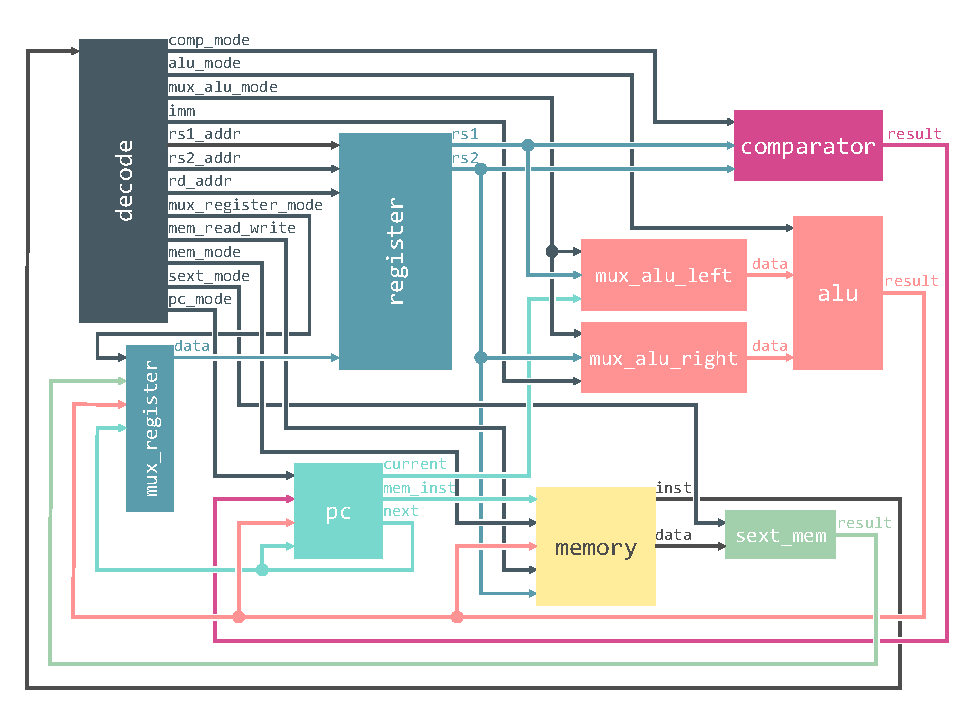
\includegraphics[scale=1]{img/OverviewCPU.pdf}
        \caption{Gesamtübersicht des Softcores}
        \label{fig:cpu_overview}
    \end{figure}


    \section{Steuerwerk}

        Die Dekodiereinheit wid im Verbund mit dem \textit{Programm Counter (PC)} (Siehe \ref{lab:pc}) auch Steuerwerk genant.

        \begin{figure}[H]
            \centering
            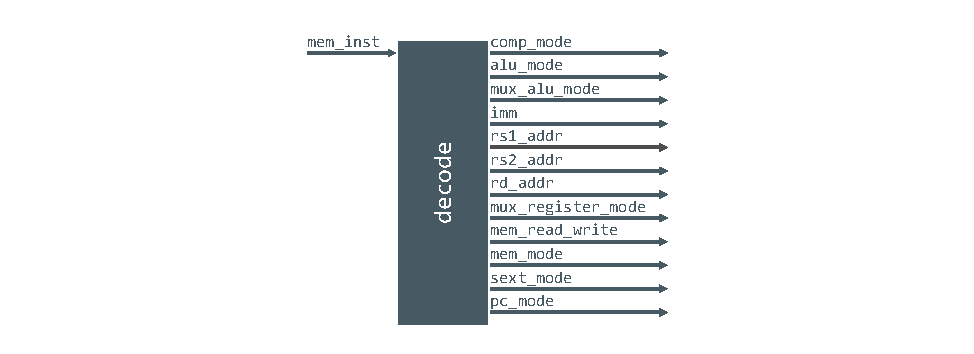
\includegraphics[scale=1]{img/block_decode.pdf}
            \caption{Dekodiereinheit}
            \label{fig:decode}
        \end{figure}

        \subsection{Dekodiereinheit}
            
            Die Dekodiereinheit ist dafür zuständig die Instruktionen aus dem Speicher zu interpretieren und die notwendigen
            Steuerleitungen zu setzen.
            Hierfür ist die Einheit direkt über den 32 Bit Instruktionbus mit dem Speicher verbunden.

        \subsection{Programm Counter (PC)}\label{lab:pc}

            \begin{figure}[H]
                \centering
                
\includegraphics[scale=1]{img/block_pc.pdf}
                \caption{Befehlszählers}
                \label{fig:pc}
            \end{figure}

            Der Befehlszähler steuert den Programmablauf und speichert in einem 32 Bit Register
            die aktuelle Adresse der Instruktion im Programspeicher.
            In jedem Taktzyklus wird die Adresse um ein Wort (32 Bit) erhöht und zeigt somit
            auf den nächsten Befehl. Dieser kann wieder von der Dekodiereinheit dekodiert werden
            und es können die Steuerleitungen gesetzt werden. Der Befehlszähler kann jedoch nicht nur
            inkrementiert sondern auch überschrieben werden.
            \newpage
            \lstinputlisting[style=vhdl,linerange={37-47},caption={Prozess des Befehlszählers}]{../../CPU/Design/src/pc/pc.vhd}

        \subsection{Branch}

            \begin{figure}[H]
                \centering
                
\includegraphics[scale=1]{img/block_comparator.pdf}
                \caption{Vergleichswerk}
                \label{fig:alu}
            \end{figure}

            Wenn eine Anweisung zur Ablaufsteuerung auf Programmebene
            ausgeführt werden soll, muss zunächst die Bedingung geprüft werden
            und dann ggfs. eine Instruktion ausgeführt werden,
            die nicht sequentiell hinter der aktuellen im Speicher liegt.
            Dies nennt man einen Zweig (englisch: Branch). Ein Zweig erfordert zusätzliche Logik in Steuerwerk 
            und wird durch eine Vergleichseinheit realisiert.
            Diese Einheit vergleicht zwei 32 Bit Daten (Links und Rechts) und liefert ein boolesches Ergebnis (ein Bit).
            Tabelle \ref{tab:comp-states} zeigt welche Vergleichsoperatoren zu Verfügung stehen.

            \begin{center}
                \begin{longtable}{| l | l | }
                    \hline
                        Zustand & Operation \\
                    \hline
                        COMP\_EQUAL & signed(links) == signed(rechts) \\
                    \hline
                        COMP\_NOT\_EQUAL & signed(links) != signed(rechts) \\
                    \hline
                        COMP\_LESS\_THEN & signed(links) < signed(rechts) \\
                    \hline
                        COMP\_GREATER\_EQUAL & signed(links) >= signed(rechts) \\
                    \hline
                        COMP\_LESS\_THEN\_U & unsigned(links) < unsigned(rechts) \\
                    \hline
                        COMP\_GREATER\_EQUAL\_U & unsigned(links) >= unsigned(rechts) \\
                    \hline
                    \caption[Zustandstabelle Vergleichswerk]{Zustandstabelle Vergleichswerk}
                    \label{tab:comp-states}
                \end{longtable}
            \end{center}
                


    \section{Register}

        \begin{figure}[H]
            \centering
            
\includegraphics[scale=1]{img/block_register.pdf}
            \caption{Registereinheit}
            \label{fig:register}
        \end{figure}


        \subsection{Registereinheit} 
            Die Registereinheit bildet 32 Register mit einer Breite von 32 Bit ab \cite{riscv-isa-specs}[2.1].
            Dabei kann in einem Taktzyklus auf zwei Register (rs1 und rs2) lesend und auf einem Register (rd) schreibend zugegriffen werden.
            Die \textit{ISA} besagt zudem, dass Register x0 immer Nullen liefern soll und nicht überschrieben werden darf \cite{riscv-isa-specs}[2.1].
            Dies wird durch eine Abfrage der Adresse im Prozess gesteuert. Falls das Zielregister, das Nullregister sein sollte werden die Werte
            nicht in das Zielregister übernommen.
            \lstinputlisting[style=vhdl,linerange={47-55},caption={Prozess der Registereinheit}]{../../CPU/Design/src/registers/registers.vhd}

        \subsection{Register Multiplexer}

            \begin{figure}[H]
                \centering
                
\includegraphics[scale=1]{img/block_mux_register.pdf}
                \caption{Register Multiplexer}
                \label{fig:register_mux}
            \end{figure}


            Die Eingangsdaten werden instruktionsabhängig augewählt und in das Zielregister (rd) geschrieben.
            Dies geschieht in einem vorgeschaltetem Multiplexer. Die Dekodiereinheit setzt dabei die notwendigen Steuerleitungen.
            Als Auswahlmöglichkeiten der Daten stehen die \textit{ALU}, der Speicher, der nächste Befehlszähler (PC + 4).
            Als gesonderte Absicherung dient der \textit{MUX\_REG\_ZERO} Zustand.
            Dieser wird standardmäßig beim initialisieren gesetzt und soll ein Überschreiben von Daten verhindern wenn z.B.
            eine unbekannte Instruktion ausgeführt werden soll.
            \lstinputlisting[style=vhdl,linerange={28-39},caption={Prozess des register Multiplexers}]{../../CPU/Design/src/registers/mux_register.vhd}

    \section{Arithmetic logic unit (ALU)}

        \begin{figure}[H]
            \centering
            
\includegraphics[scale=1]{img/block_alu.pdf}
            \caption{ALU}
            \label{fig:alu}
        \end{figure}

        \subsection{Rechenwerk}
            Die \textit{Arithmetic logic unit (ALU)} ist das Rechenwerk und berechnet arith­me­tisch sowie logische Operationen.
            Dabei werden nicht nur Register-Register Berechnungen sondern auch Immediate- sowie Sprungberechnungen
            basierend auf dem aktuellen Befehlszähler durchgeführt.
            Da der Befehlssatz nur Integer Operationen erlaubt können auch nur diese in Hardware umgesetzt werden \cite{riscv-isa-specs}[2.4].
            Ebenfalls fehlen der \textit{ISA} Multiplikation sowie Division.
            Diese können über Softwarebibliotheken mit Addition und Subtraktion durchgeführt werden,
            benötigen jedoch mehr Instruktionen, verbrauchen dadurch mehr Programmspeicher und schlagen sich somit negativ auf die Performanz aus.

        \subsection{Rechenwerk Multiplexer}

            \begin{figure}[H]
                \centering
                
\includegraphics[scale=1]{img/block_mux_alu_left.pdf}
                \caption{Linker ALU Multiplexer}
                \label{fig:alu_mux_left}
            \end{figure}

            \begin{figure}[H]
                \centering
                
\includegraphics[scale=1]{img/block_mux_alu_right.pdf}
                \caption{Rechter ALU Multiplexer}
                \label{fig:alu_mux_right}
            \end{figure}

            Die beiden Rechenwerk Multiplexer (Links und Rechts) steuern die Eingangsdaten des Rechenwerks und bestimmen somit welche Daten
            berechnet werden. Die Steuerleitungen werden dabei instruktionsabhängig in der Dekodiereinheit gesetzt.
            Beide Multiplexer teilen die selben Zustände, reagieren jedoch anders.
            Tabelle \ref{tab:alu-mux} zeigt die verschiedenen Zustände und die damit verbundenen Eingangsdaten für die \textit{ALU}.


            \begin{center}
                \begin{longtable}{| l | c | c | l |}
                    \hline
                        Zustand & Linker Operand & Rechter Operand & Berechnung \\
                    \hline
                        MUX\_ALU\_RS1\_RS2 & rs1 & rs2 & Register-Register \\
                    \hline
                        MUX\_ALU\_RS1\_IMM & rs1 & immediate &  Register-Immediate\\
                    \hline
                        MUX\_ALU\_PC\_IMM & pc & immediate & Sprung \\
                    \hline
                        MUX\_ALU\_PC\_RS2 & pc & rs2 & Sprung \\
                    \hline
                    \caption[Zustandstabelle ALU Multiplexer]{Zustandstabelle ALU Multiplexer}
                    \label{tab:alu-mux}
                \end{longtable}
            \end{center}

            \lstinputlisting[style=vhdl,linerange={26-37},caption={Prozess des linken Rechenwerk Multiplexers}]{../../CPU/Design/src/alu/mux_alu_left.vhd}
            \lstinputlisting[style=vhdl,linerange={27-38},caption={Prozess des rechten Rechenwerk Multiplexers}]{../../CPU/Design/src/alu/mux_alu_right.vhd}

    \section{Memory}\label{lab:memory}

        Durch die gewählte \textit{modifizierte Havard-Architektur} und den \textit{Ein-Zyklus-Ansatz}
        muss sicherstegestellt werden, dass in einem Taktzyklus sowohl Instruktion gelesen als auch die damit verbundenen Daten
        gelesen bzw. geschrieben werden können. Dies wird dadurch ermöglicht, dass die Instruktionen zur steigenden Taktflanke
        gelesen und die Daten zur fallenden Taktflanke gelesen bzw. geschrieben werden.
        Dies ist nur möglich, da die Taktzeit mehr als doppelt so lang ist, wie die Zeit die benötigt wird um eine Speicheroperation
        durchzuführen \cite{intel-cyc10lp-device-datasheet}[Tabelle 23].

        \begin{equation}
            \frac{1}{12Mhz} > 2\cdot\frac{1}{238Mhz}
        \end{equation}


        \begin{figure}[H]
            \centering
            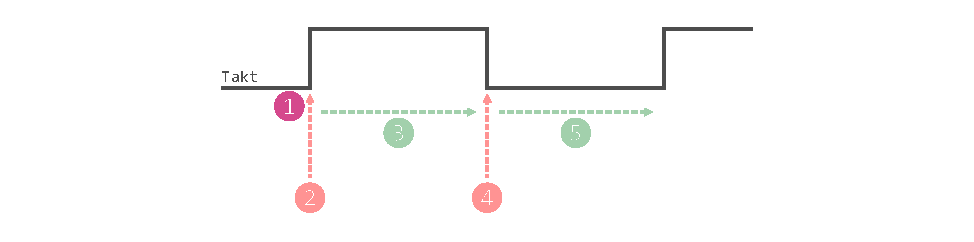
\includegraphics[scale=1]{img/Timing_Memory.pdf}
            \caption{Taktflanken am Speicher}
            \label{fig:timing_memory}
        \end{figure}

         \begin{enumerate}
             \item Neue Instruktionsadresse muss bereits anliegen
             \item Instruktion wird aus Speicher gelesen / Steuerwerk setzt Kontrollsignale
             \item Instruktion wird ausgeführt / Adresse für Daten wird berechnet.
             \item Daten werden an berechneter Adresse geschrieben bzw. gelesen
             \item Gelesen Daten werden durch ALU verrechnet und in Zielregister geschrieben. / Daten werden aus Register in Speicher geschrieben
         \end{enumerate}

            
        \subsection{Byte-Adressierung}
            Auch wenn die Speicherausrichtung natürlich ist (Siehe \ref{lab:mem-order}), fordert der Befehlssatz eine Byte-Adressierung,
            sodass auf einzelne Bytes in einem Wort zugegriffen werden kann. Leider erlauben das die \textit{M9K} Speicherblöcke nicht.
            Aus diesem Grund wurden vier Speicherpartitionen erstellt die jeweils ein Viertel des gesamten Speichers ausmachen.
            Soll nur ein einzelnes Byte gelesen bzw. geschrieben werden, wird nur eine Speicherpartition adressiert.
            Bei einem \textit{half-Word} werden hingegen zwei Partitionen ausgelesen. Dabei wird sichergestellt,
            dass nicht über die natürliche Ausrichtung hinweg adressiert werden kann.
            Eine Speicherpartition wird durch \textit{memory\_byte.vhd} repräsentiert und wird durch die \textit{Megafunction} erstellt.
            Somit wird gewährleistet, dass die \textit{M9K}-Blöcke des \textit{FPGA's} benutzt werden.
            In \textit{memory\_word.vhd} wird die Logik definiert, die zuständig ist um bei jeweiliger Adresse die 
            richtige Speicherpartition zu adressieren.
            Für Instruktionen und Daten stehen insgesamt 65535 Bytes zu Verfügung.

        \subsection{Initialisierung}\label{lab:mif}
            Die Initialisierung erfolgt über ein \textit{Memory initialization files (MIF)} \cite{intel-mif}.
            Die einfache \textit{Key-Value-}Syntax (Tabelle \ref{tab:mif-syntax}) erlaubt eine Abbildung der Speicheradressen sowie deren korrespondierenden Daten.
            Die eigentliche Initialisierung erfolgt entweder zur Synthesezeit oder zur Laufzeit über den Quartus Assembler (Siehe \ref{lab:flash-softcore}).
            Listing \ref{lst:mif-example} zeigt ein Beispiel MIF.
            \begin{center}
                \begin{longtable}{| l | l |}
                    \hline
                        Schlüsselwort & Wert\\
                    \hline
                        DEPTH & Speichergröße in Words\\
                    \hline
                        WIDTH & Wordgröße\\
                    \hline
                        ADDRESS\_RADIX & Repräsentation der Adressen\\
                    \hline
                        DATA\_RADIX & Repräsentation der Daten\\
                    \hline
                        CONTENT & Adress-Daten Paare\\
                    \hline
                    \caption[MIF Syntax]{MIF Syntax}
                    \label{tab:mif-syntax}
                \end{longtable}
            \end{center}

            \lstinputlisting[style=mif,caption={Beispiel MIF},label=lst:mif-example]{src/ram.mif.ex}


        \subsection{Sign-Extender}

            \begin{figure}[H]
                \centering
                
\includegraphics[scale=1]{img/block_sext.pdf}
                \caption{Vorzeichenerweiterung}
                \label{fig:sext}
            \end{figure}

            Die Vorzeichenerweiterung wird verwendet um ausgelesene Werte aus dem Speicher auf Wordgröße
            zu erweitern. Grund dafür ist, dass Werte kleinerer Breite ausgelesen werden können wie z.B. ein
            Byte oder Halfword. Da die Register jedoch alle mit einer fixen Wordbreite von 32 Bit arbeiten muss ggfs.
            aufgefüllt werden. Ob mit Nullen oder Einsen aufgefüllt wird, ist abhängig von der Operation und wird über den
            \textit{sext\_mode} durch den Dekoder eingestellt.
            
    \section{IO}

        Die Anbindung von Peripherie erfolgt über \textit{Memory-Mapping}.
        Dabei wird ein zusätzlicher Bereich im Speicher nur für Peripherie reserviert (Abbildung \ref{fig:io}).
        Je nachdem welcher Bereich adressiert wird, werden Daten geschrieben bzw. gelesen
        oder die Peripherie angesteuert. Darüber entscheidet der Prozess \textit{ram\_or\_ext}
        in der \textit{memory.vhd} (Listing \ref{lst:memory}).

        \begin{figure}[H]
            \centering
            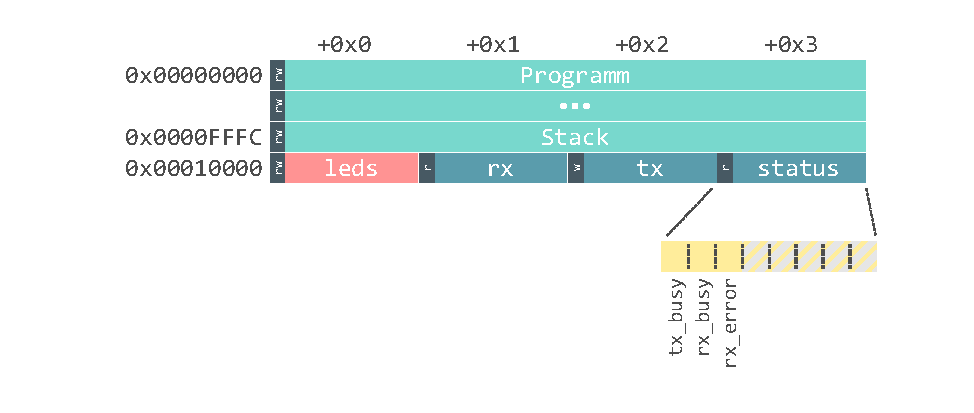
\includegraphics[scale=1]{img/memory.pdf}
            \caption{Speicher mit IO Bereich}
            \label{fig:io}
        \end{figure}

        \lstinputlisting[style=VHDL,caption={Adressaufteilung im Speicher},linerange={56-70},label=lst:memory]{../../CPU/Design/src/memory/memory.vhd}
        \newpage
        \lstinputlisting[style=VHDL,caption={Leseprozess für die Peripherie},linerange={39-47},label=lst:peripherie-read]{../../CPU/Design/src/io/peripherie.vhd}
        \lstinputlisting[style=VHDL,caption={Schreibeprozess für die Peripherie},linerange={50-63},label=lst:peripherie-write]{../../CPU/Design/src/io/peripherie.vhd}

        \subsection{LED}
            Es stehen acht LED's auf dem \textit{FPGA}-Board zur Verfügung die über den erweiterten Speicherbereich
            angesteuert werden können. Der Status der LED's kann hierbei gesetzt sowie abgefragt werden.
            Dazu dienen die beiden Prozesse in \textit{peripherie.vhd} (Siehe Listing \ref{lst:peripherie-read} und \ref{lst:peripherie-write}).

        \subsection{UART}
            Zusätzlich steht eine \textit{UART}-Schnittstelle zu Verfügung die es erlaubt Byteweise Daten
            zu senden oder empfangen.
            Dabei wurde das Modul im Rahmen dieser Arbeit nicht entwickelt und ist somit ein Fremdmodul \cite{vhdl-uart}.
            Es funktioniert jedoch nach dem gleichen Prinzip des \textit{Memory-Mappings}.
            Wie Listing \ref{lst:peripherie-read} und \ref{lst:peripherie-write} zeigen,
            besteht es aus drei Adressbereichen (Status, RX und TX) aus denen gelesen bzw. in die geschrieben werden kann.
            

